For the standard model processes, we account for the same systematic
uncertainties as the SM Higgs search~\cite{HWWHCP2012},
for both normalisation and template shapes.
For the exotic resonance signals, such as the spin-2 
graviton ($2_\text{min}^+$), we apply additional 
shape systematics to account for missing higher order effects in JHUgen. 

As discussed in Section~\ref{sec:jhugenval}, we reweight the $gg\to \text{Graviton}\to WW$
signal template.
The weight for each bin in ($m_T, m{\ell\ell}$) is derived by comparing
the $m_T-m_{\ell\ell}$ templates for the standard model Higgs hypothesis
generated with JHUGen-Pythia and Powheg-Pythia.
We then consider the JHUGen-Pythia 
predictions without reweighting as the $+1\sigma$ deviation from the central shape.
The corresponding $-1\sigma$ variation is then derived from the mirrored difference between 
the central and the $+1\sigma$ difference. 
Figure~\ref{fig:xwwshapevar} shows the central and $\pm1\sigma$ variations 
of the $gg\to \text{Graviton}\to WW$. 

\vspace{20pt}


%%%%%%%%%%%%%%%%%%%%%%%%%%%%%%%%%%%%%%%%%%%%%
\begin{figure}[!hbtp]
\centering
\label{subfig:xwwshapevar}
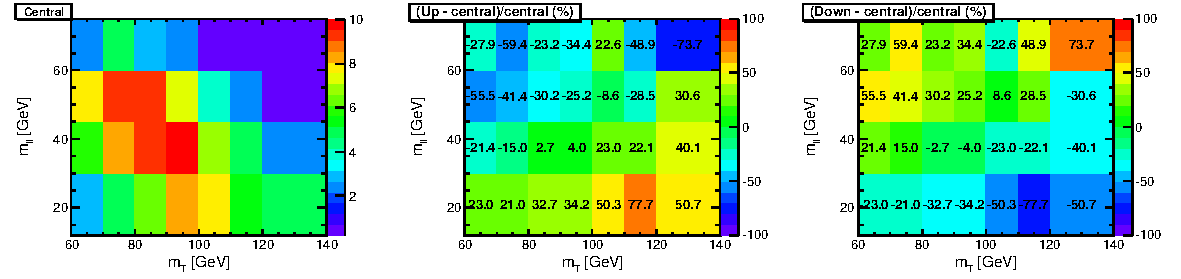
\includegraphics[width=1.05\textwidth]{figures/xww_ggHshapevar.pdf}
\caption{The shape variations for the $gg\to \text{Graviton}\to WW$. 
}
\label{fig:xwwshapevar}
\end{figure}
%%%%%%%%%%%%%%%%%%%%%%%%%%%%%%%%%%%%%%%%%%%%%
